\chapter{Cinética de electrodo y electroanálisis}\label{ch:b3:electrode-kinetics}

Una gota de sangre sobre una tira de plástico, cinco segundos, un número: el medidor de
glucosa que millones de personas usan varias veces al día es una celda
electroquímica, y lo que mide no es una tensión sino una corriente. Una \omterm{def:b3:complex-kinetics:enzyme}{enzima} oxida
la glucosa, un complejo de hierro disuelto lleva los electrones a un electrodo de
carbono, y la corriente que circula está fijada por la rapidez con que ese complejo difunde
hasta el electrodo, y por tanto por su concentración. Este capítulo explica por qué
los electrones atraviesan una interfase deprisa o despacio (la \omterm{thm:b3:electrode-kinetics:butler-volmer}{ecuación de Butler--Volmer}), cómo
el transporte de materia limita la corriente, y cómo la \omterm{def:b3:electrode-kinetics:cv}{voltamperometría cíclica} y los demás
métodos electroanalíticos convierten corrientes en concentraciones, constantes de velocidad
y mecanismos.

\begin{recall}
El volumen del primer año definió el potencial de electrodo, el potencial estándar, la
ecuación de Nernst, los electrodos de referencia y las semipilas. El volumen del segundo año
introdujo las curvas intensidad--potencial con sus corrientes anódica y catódica,
los electrodos de trabajo y los contraelectrodos, las sobretensiones, los sistemas rápidos y lentos, la
capa de difusión y la corriente límite; los coeficientes de actividad y la fuerza
iónica; las rectas de calibrado, el método de las adiciones estándar y el límite de
detección. El \cref{ch:b3:rate-theories} dio la \omterm{def:b3:rate-theories:tst}{teoría del estado de transición}. De la
física: las leyes de Fick de la difusión, la ecuación de Poisson y los condensadores.
\end{recall}

\begin{omfigure}
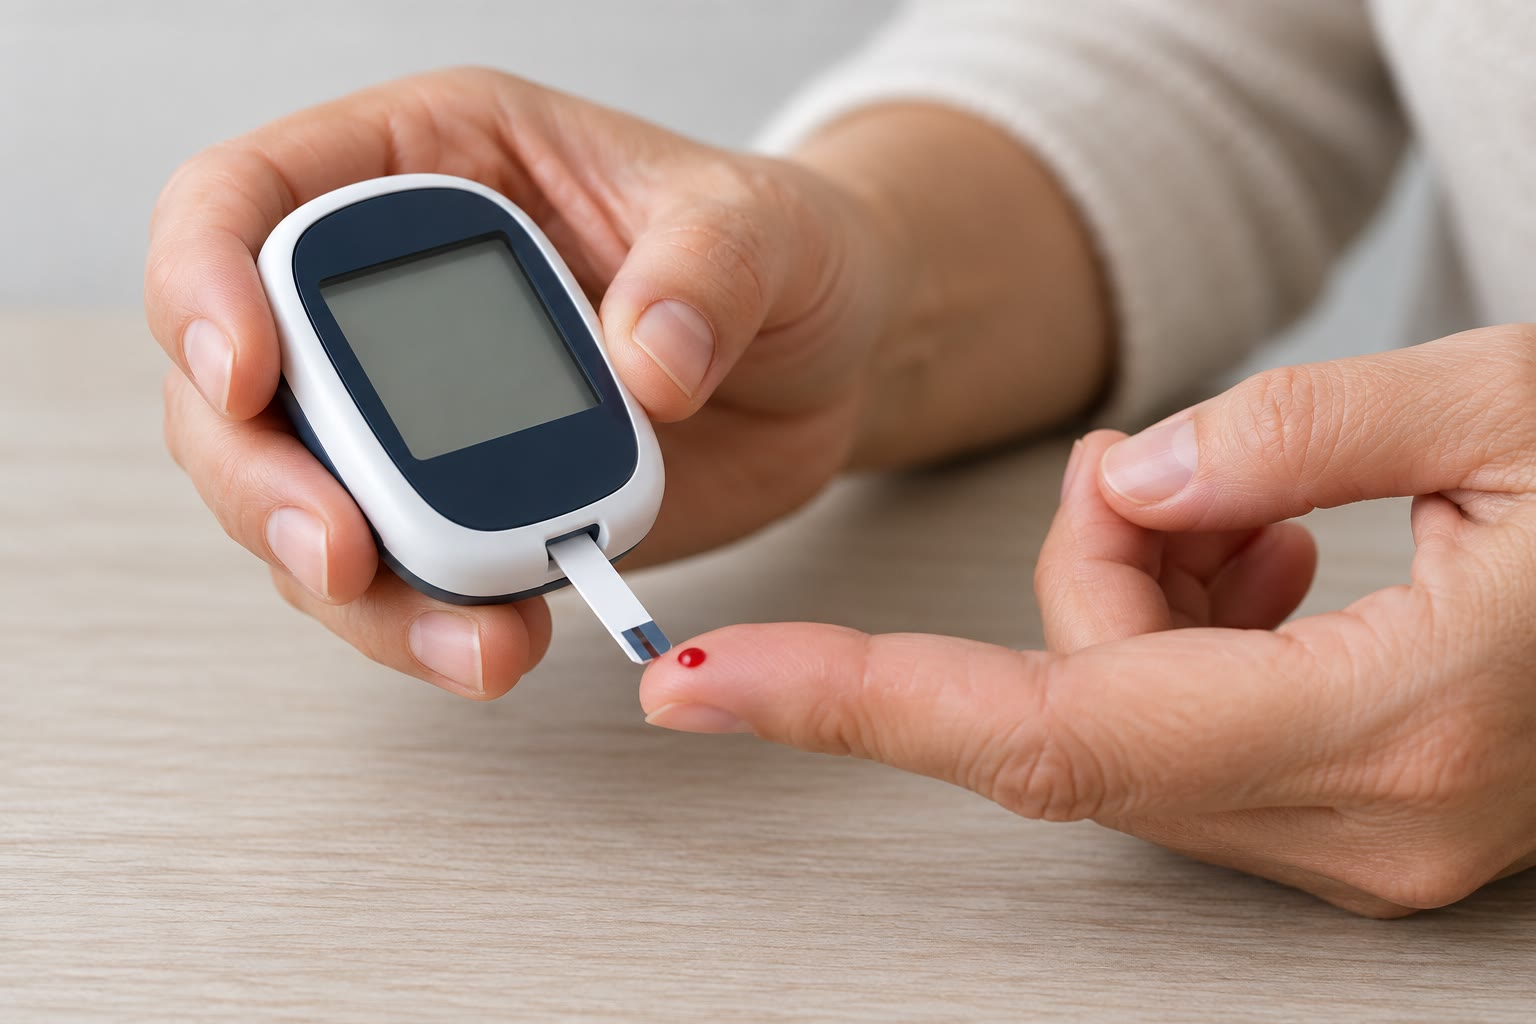
\includegraphics[width=0.6\linewidth]{images/book4/ai/b3-15-glucose-meter.jpg}

{\small Un medidor de glucosa en sangre: la tira lleva una diminuta celda de tres electrodos
con una \omterm{def:b3:complex-kinetics:enzyme}{enzima} y un mediador redox; el medidor aplica un potencial y lee una
corriente.}
\end{omfigure}

\section{La interfase electrodo--disolución}

Un metal sumergido en una disolución de electrolito lleva una carga superficial, y la
disolución responde con una carga igual y opuesta formada por un exceso de iones
de un signo. Las dos capas de carga forman un condensador de espesor molecular.

\begin{definition}[Doble capa eléctrica]\label{def:b3:electrode-kinetics:double-layer}
La \emph{doble capa eléctrica}\index{doble capa electrica@doble capa eléctrica} es la
disposición de la carga en una interfase electrodo--disolución: la carga del
metal y la carga iónica que la compensa en la disolución. Su parte compacta, la
\emph{capa de Helmholtz}\index{capa de Helmholtz}, es la capa de iones y de moléculas de disolvente
en contacto con la superficie; su \emph{capa difusa}\index{capa difusa}
es la región situada más allá, donde la agitación térmica reparte el exceso de iones sobre
una distancia del orden de la \emph{longitud de Debye}\index{longitud de Debye} $\kappa^{-1}$. La
\emph{capacidad de la doble capa}\index{capacidad de la doble capa} $C_{\mathrm{dl}}$ es la carga
almacenada por unidad de área y por voltio de potencial a través de la interfase.
\end{definition}

\begin{proposition}[Longitud de Debye]\label{prop:b3:electrode-kinetics:debye-length}
En una disolución de fuerza iónica $I$ (en \unit{mol.m^{-3}}) y permitividad relativa
$\varepsilon_r$, un potencial pequeño $\varphi_0$ en el electrodo decae en la disolución como
$\varphi = \varphi_0\eu^{-\kappa x}$, con
\[
  \kappa^{-1} = \sqrt{\frac{\varepsilon_r\varepsilon_0RT}{2F^2I}} .
\]
\end{proposition}

\begin{proof}
La ecuación de Poisson (de la física) relaciona el potencial con la densidad de carga:
$\dd^2\varphi/\dd x^2 = -\rho/\varepsilon_r\varepsilon_0$. Cada ion obedece a la \omterm{def:b3:partition-functions:boltzmann}{distribución de Boltzmann} en el
potencial: $c_i = c_i^{\circ}\eu^{-z_iF\varphi/RT}$, luego $\rho = F\sum_iz_ic_i^{\circ}\eu^{-z_iF\varphi/RT}$. Para $F\varphi \ll RT$,
$\eu^{-z_iF\varphi/RT} \approx 1 - z_iF\varphi/RT$; los términos de orden cero se cancelan por la electroneutralidad,
y $\rho \approx -(F^2/RT)\sum_iz_i^2c_i^{\circ}\,\varphi = -(2F^2I/RT)\varphi$. Por tanto, $\dd^2\varphi/\dd x^2 = \kappa^2\varphi$, cuya
solución que se anula lejos es $\varphi_0\eu^{-\kappa x}$.
\end{proof}

\begin{example}[El espesor de la doble capa]\label{ex:b3:electrode-kinetics:debye}
% ledger: eps:H2O.25C, const:eps0, const:F, const:R
En agua a \qty{298.15}{K} ($\varepsilon_r = 78.4$) con \qty{0.10}{mol/L} de una sal 1:1 ($I = \qty{100}{mol.m^{-3}}$),
$\kappa^{-1} = \sqrt{78.4 \times \num{8.854e-12} \times 2479/(2 \times 96\,485^2 \times 100)} = \qty{0.96}{nm}$; con \qty{1.0}{mmol/L},
diez veces más. Un \omterm{def:b3:electrode-kinetics:transport}{electrolito soporte} comprime la \omterm{def:b3:electrode-kinetics:double-layer}{capa difusa} hasta unos pocos
diámetros moleculares.
\end{example}

La \omterm{def:b3:electrode-kinetics:double-layer}{capa difusa} se comporta como un condensador cuyas placas están separadas $\kappa^{-1}$: su
capacidad por unidad de área a bajo potencial es $\varepsilon_r\varepsilon_0\kappa$ (el resultado de
Gouy--Chapman; su dependencia del potencial se admite). En serie con la
capa compacta de Helmholtz, da la $C_{\mathrm{dl}}$ medida, del orden de decenas de
microfaradios por centímetro cuadrado (el modelo de Stern). Siempre que cambia el potencial, este condensador
se carga: un barrido a $v$ voltios por segundo consume una corriente de carga $C_{\mathrm{dl}}Av$ que
no lleva química alguna y se suma a toda medida voltamperométrica.

\begin{omfigure}
\begin{tikzpicture}[font=\small, >=Stealth]
  \fill[black!25] (-1.0,0) rectangle (0,3.2);
  \node[rotate=90] at (-0.5,1.6) {metal};
  \foreach \y in {0.3,0.8,...,2.9}{\node[font=\scriptsize] at (-0.15,\y) {$-$};}
  \foreach \y in {0.35,0.95,1.55,2.15,2.75}{\draw[omDef, fill=omDef!20] (0.3,\y) circle (0.18); \node[font=\scriptsize] at (0.3,\y) {$+$};}
  \draw[black!50, dashed] (0.55,0) -- (0.55,3.2);
  \node[font=\scriptsize, anchor=south, align=center] at (0.45,3.25) {plano de\\ Helmholtz};
  \foreach \x/\y/\s in {1.1/0.6/+, 1.4/2.2/+, 1.9/1.3/+, 2.3/2.7/-, 2.6/0.5/+, 3.1/1.8/+, 3.5/0.9/-, 3.9/2.4/+, 4.4/1.4/-, 4.8/0.4/+, 5.1/2.8/-, 5.4/1.9/+}{
    \draw[black!60, fill=white] (\x,\y) circle (0.15); \node[font=\scriptsize] at (\x,\y) {$\s$};}
  \node[font=\scriptsize, anchor=south] at (3.2,3.25) {capa difusa};
  \draw[->] (0,-2.1) -- (6.0,-2.1) node[anchor=north east] {$x$};
  \draw[->] (0,-2.1) -- (0,-0.3) node[anchor=east] {$|\varphi|$};
  \draw[omThm, thick] (0,-0.5) -- (0.55,-1.0) plot[domain=0.55:5.8, samples=40] (\x,{-2.1+1.1*exp(-(\x-0.55)/1.2)});
  \draw[black!40, dashed] (0.55,-2.1) -- (0.55,-0.4);
  \node[omThm, anchor=south west] at (1.3,-1.6) {$|\varphi(x)|$};
  \draw[<->, black!60] (0.55,-2.5) -- (1.75,-2.5) node[midway, below, font=\scriptsize] {$\sim\kappa^{-1}$};
\end{tikzpicture}

{\small La \omterm{def:b3:electrode-kinetics:double-layer}{doble capa eléctrica} (modelo de Gouy--Chapman--Stern, esquema): un
metal cargado negativamente, una capa compacta de cationes en el plano de Helmholtz
y una \omterm{def:b3:electrode-kinetics:double-layer}{capa difusa} en la que los cationes superan en número a los aniones a lo largo de unas pocas \omterm{def:b3:electrode-kinetics:double-layer}{longitudes de Debye}.
Abajo, la magnitud del potencial (negativo, como la carga del metal) disminuye
linealmente a través de la capa compacta y después exponencialmente en la \omterm{def:b3:electrode-kinetics:double-layer}{capa difusa}.}
\end{omfigure}

\section{Cinética de la transferencia electrónica}

Se considera la reducción $\mathrm{O} + n\,\mathrm{e}^- \to \mathrm{R}$ en un electrodo mantenido al potencial $E$,
cuyo potencial de equilibrio para la disolución del seno sería $E_{\mathrm{eq}}$. La
sobretensión es $\eta = E - E_{\mathrm{eq}}$.

\begin{definition}[Densidad de corriente de intercambio, coeficiente de transferencia, constante de velocidad estándar]\label{def:b3:electrode-kinetics:exchange}
En el equilibrio, las corrientes anódica y catódica son iguales y opuestas; su
módulo común por unidad de área es la \emph{densidad de corriente de
intercambio}\index{densidad de corriente de intercambio} $j_0$. El \emph{coeficiente de transferencia}
\index{coeficiente de transferencia} $\alpha$ ($0 < \alpha < 1$) es la fracción de la
energía eléctrica $nF\eta$ que rebaja la barrera de la reacción catódica. La
\emph{constante de velocidad estándar}\index{constante de velocidad estandar@constante de velocidad estándar} $k^\circ$ es el valor común
de las constantes de velocidad catódica y anódica en el potencial formal $E^{\circ\prime}$.
\end{definition}

\begin{theorem}[Ecuación de Butler--Volmer]\label{thm:b3:electrode-kinetics:butler-volmer}
Si las concentraciones en la superficie son iguales a las del seno de la disolución (sin limitación
por transporte de materia), la densidad de corriente para la sobretensión $\eta$ es, contando
positivas las corrientes anódicas,
\[
  j = j_0\bigl[\eu^{(1 - \alpha)f\eta} - \eu^{-\alpha f\eta}\bigr], \qquad f = \frac{nF}{RT}.
\]
Es la \emph{ecuación de Butler--Volmer}\index{ecuacion de Butler--Volmer@ecuación de Butler--Volmer}.
\end{theorem}

\begin{proof}
Según la \omterm{def:b3:rate-theories:tst}{teoría del estado de transición}, las constantes de velocidad catódica y anódica son
$k_{\mathrm c} = A\eu^{-\Delta G_{\mathrm c}^{\ddagger}/RT}$ y $k_{\mathrm a} = A\eu^{-\Delta G_{\mathrm a}^{\ddagger}/RT}$. Cambiar el potencial del electrodo en $\delta E$
cambia la energía de Gibbs de la reacción $\mathrm{O} + n\,\mathrm{e}^- \to \mathrm{R}$ en $nF\,\delta E$ (los electrones
del metal ganan $-nF\,\delta E$ de energía eléctrica). Se supone, a primer orden, que una
fracción $\alpha$ de este cambio va a la barrera catódica y el resto a la
anódica: $\Delta G_{\mathrm c}^{\ddagger} \to \Delta G_{\mathrm c}^{\ddagger} + \alpha nF\,\delta E$, $\Delta G_{\mathrm a}^{\ddagger} \to \Delta G_{\mathrm a}^{\ddagger} - (1 - \alpha)nF\,\delta E$. Midiendo $\delta E$
desde el potencial de equilibrio, donde las dos corrientes valen ambas $j_0$ en
módulo, se obtiene $j_{\mathrm c} = j_0\eu^{-\alpha f\eta}$ y $j_{\mathrm a} = j_0\eu^{(1 - \alpha)f\eta}$; la corriente neta es su
diferencia.
\end{proof}

\begin{corollary}[Resistencia de transferencia de carga]\label{cor:b3:electrode-kinetics:linear}
Para $|\eta| \ll RT/nF$, $j = j_0f\eta$: la interfase se comporta como una resistencia
$R_{\mathrm{ct}} = RT/(nFi_0)$, con $i_0 = j_0A$.
\end{corollary}

\begin{proof}
Se desarrollan ambas exponenciales a primer orden: $j = j_0[(1 - \alpha)f\eta + \alpha f\eta] = j_0f\eta$; luego
$\eta/i = 1/(fi_0)$.
\end{proof}

\begin{corollary}[Ecuación de Tafel]\label{cor:b3:electrode-kinetics:tafel}
Para $\eta \ll -RT/nF$ (una sobretensión fuertemente catódica), el término anódico es
despreciable y
\[
  \eta = \frac{2.303\,RT}{\alpha nF}\bigl(\log j_0 - \log|j|\bigr):
\]
$\log|j|$ es lineal en $\eta$, con una pendiente de $1/(\text{\qty{118}{mV}})$ por década a \qty{298}{K} para $\alpha = 0.5$, $n =
1$. Es la \emph{ecuación de Tafel}\index{ecuacion de Tafel@ecuación de Tafel}.
\end{corollary}

\begin{proof}
$|j| = j_0\eu^{-\alpha f\eta}$, luego $\ln|j| = \ln j_0 - \alpha f\eta$; se pasa a logaritmos decimales.
\end{proof}

\begin{definition}[Resistencia de transferencia de carga, pendiente de Tafel]\label{def:b3:electrode-kinetics:charge-transfer}
La \emph{resistencia de transferencia de carga}\index{resistencia de transferencia de carga} de un
electrodo es $R_{\mathrm{ct}} = (\partial\eta/\partial i)_{\eta = 0}$. La \emph{pendiente de Tafel}\index{pendiente de Tafel}
es la variación de la sobretensión por década de corriente en la región de Tafel,
$2.303\,RT/\alpha nF$.
\end{definition}

\begin{omfigure}
\begin{tikzpicture}
\begin{axis}[name=bv, omcv, width=0.47\linewidth, height=5.4cm, xmin=-300, xmax=300, ymin=-40, ymax=40,
  xlabel={$\eta$ / mV}, ylabel={$j/j_0$},
  legend style={font=\scriptsize, draw=none, at={(0.03,0.97)}, anchor=north west}, legend cell align=left]
\addplot[omDef, thick] table[x=eta_mV, y=a3] {figdata/out/bachelor-3-butler-volmer.dat};
\addplot[black, thick] table[x=eta_mV, y=a5] {figdata/out/bachelor-3-butler-volmer.dat};
\addplot[omThm, thick] table[x=eta_mV, y=a7] {figdata/out/bachelor-3-butler-volmer.dat};
\legend{$\alpha = 0.3$, $\alpha = 0.5$, $\alpha = 0.7$}
\draw[black!30] (axis cs:-300,0) -- (axis cs:300,0) (axis cs:0,-40) -- (axis cs:0,40);
\end{axis}
\begin{axis}[at={(bv.east)}, anchor=west, xshift=1.2cm, omcv, width=0.47\linewidth, height=5.4cm,
  xmin=-300, xmax=300, ymin=-1.5, ymax=4, xlabel={$\eta$ / mV}, ylabel={$\log|j/j_0|$},
  unbounded coords=jump]
\addplot[omDef, thick] table[x=eta_mV, y=l3] {figdata/out/bachelor-3-butler-volmer.dat};
\addplot[black, thick] table[x=eta_mV, y=l5] {figdata/out/bachelor-3-butler-volmer.dat};
\addplot[omThm, thick] table[x=eta_mV, y=l7] {figdata/out/bachelor-3-butler-volmer.dat};
\draw[black!40, dashed] (axis cs:-300,2.54) -- (axis cs:0,0);
\draw[black!50] (axis cs:-200,1.85) -- (axis cs:-120,3.3) node[anchor=south, font=\scriptsize, inner sep=1pt] {pendiente $1/(\qty{118}{mV})$};
\end{axis}
\end{tikzpicture}

{\small La \omterm{thm:b3:electrode-kinetics:butler-volmer}{ecuación de Butler--Volmer} ($n = 1$, \qty{298}{K}) para tres \omterm{def:b3:electrode-kinetics:exchange}{coeficientes de
transferencia}. Izquierda: la corriente es lineal en $\eta$ cerca del equilibrio (la
\omterm{def:b3:electrode-kinetics:charge-transfer}{resistencia de transferencia de carga}) y exponencial más allá; $\alpha$ la hace asimétrica.
Derecha: la gráfica de Tafel, cuyas ramas rectas extrapolan a $\log|j/j_0| = 0$
en $\eta = 0$; la línea discontinua es la recta de Tafel catódica para $\alpha = 0.5$.}
\end{omfigure}

\begin{method}[Un análisis de Tafel]\label{met:b3:electrode-kinetics:tafel-analysis}
\begin{enumerate}
  \item Registrar la corriente estacionaria en función de $\eta$ en una disolución agitada, muy por debajo de la
        corriente límite (o corregir el transporte de materia).
  \item Representar $\log|i|$ en función de $\eta$; ajustar la rama lineal más allá de unos \qty{100}{mV}.
  \item La pendiente da $\alpha$ (o $1 - \alpha$ en la rama anódica); la ordenada en $\eta = 0$
        da $\log i_0$.
  \item Comprobación: cerca de $\eta = 0$, la pendiente de $i$ en función de $\eta$ es $1/R_{\mathrm{ct}} = nFi_0/RT$.
\end{enumerate}
\end{method}

Los sistemas rápidos y lentos del volumen del segundo año son los dos extremos de este
cuadro: un sistema rápido tiene una $j_0$ grande y su curva intensidad--potencial sube
bruscamente en el potencial de equilibrio; un sistema lento necesita una gran sobretensión
antes de que circule corriente alguna. La \omterm{def:b3:electrode-kinetics:exchange}{densidad de corriente de intercambio} de una misma reacción
varía en muchos órdenes de magnitud de un material de electrodo a otro:
el desprendimiento de hidrógeno es rápido sobre platino y extremadamente lento sobre mercurio.

\section{Transporte de materia}

\begin{definition}[Modos de transporte de materia]\label{def:b3:electrode-kinetics:transport}
Las especies llegan a un electrodo por \emph{migración}\index{migracion@migración}, el movimiento de los iones
en el campo eléctrico; por difusión, a favor de los gradientes de concentración; y por
\emph{convección}\index{conveccion@convección}, el movimiento de la disolución en su conjunto
(agitación, rotación, flujo). Un \emph{electrolito soporte}\index{electrolito soporte}
es una sal inerte añadida en gran exceso, que transporta casi toda
la corriente a través de la disolución, de modo que la especie electroactiva solo se desplaza por
difusión y convección.
\end{definition}

\begin{definition}[Cronoamperometría]\label{def:b3:electrode-kinetics:chronoamperometry}
La \emph{cronoamperometría}\index{cronoamperometria@cronoamperometría} registra la corriente en función del tiempo
tras un salto del potencial del electrodo.
\end{definition}

\begin{theorem}[Ecuación de Cottrell]\label{thm:b3:electrode-kinetics:cottrell}
Tras un salto de potencial en $t = 0$ hasta un valor en el que la especie electroactiva se
consume en cuanto llega a un electrodo plano de área $A$, en una disolución en
reposo con \omterm{def:b3:electrode-kinetics:transport}{electrolito soporte}, la corriente es
\[
  i = nFAc^*\sqrt{\frac{D}{\pi t}},
\]
donde $c^*$ es la concentración en el seno de la disolución y $D$ el coeficiente de difusión. Es
la \emph{ecuación de Cottrell}\index{ecuacion de Cottrell@ecuación de Cottrell}.
\end{theorem}

\begin{proof}
La concentración obedece a la segunda ley de Fick, $\partial c/\partial t = D\,\partial^2c/\partial x^2$, con $c(x, 0) = c^*$,
$c(0, t) = 0$ para $t > 0$ y $c \to c^*$ lejos. La función $c = c^*\operatorname{erf}(x/2\sqrt{Dt})$, con
$\operatorname{erf}u = \frac{2}{\sqrt\pi}\int_0^u\eu^{-s^2}\dd s$, cumple estas condiciones: $\operatorname{erf}0 = 0$, $\operatorname{erf}u \to 1$ cuando $u \to \infty$
(en $t \to 0$ para todo $x > 0$, y lejos). Con $u = x/2\sqrt{Dt}$,
$\partial c/\partial t = c^*\frac{2}{\sqrt\pi}\eu^{-u^2}\partial u/\partial t = -c^*\frac{2}{\sqrt\pi}\eu^{-u^2}\frac{u}{2t}$ y $\partial^2c/\partial x^2 = c^*\frac{2}{\sqrt\pi}(-2u)\eu^{-u^2}\frac{1}{4Dt}$: los
dos miembros de la ley de Fick coinciden. La corriente es el flujo en la superficie: $i =
nFAD(\partial c/\partial x)_{x = 0} = nFADc^*\frac{2}{\sqrt\pi}\frac{1}{2\sqrt{Dt}} = nFAc^*\sqrt{D/\pi t}$. (La unicidad de la solución se
admite.)
\end{proof}

\begin{omfigure}
\begin{tikzpicture}
\begin{axis}[name=pr, width=0.47\linewidth, height=5.2cm, xmin=0, xmax=600, ymin=0, ymax=1.08,
  axis lines=left, xlabel={$x$ / \unit{\micro m}}, ylabel={$c/c^*$},
  tick label style={font=\small}, label style={font=\small},
  legend style={font=\scriptsize, draw=none, at={(0.97,0.03)}, anchor=south east}, legend cell align=left]
\addplot[omDef, thick] table[x=x_um, y=t1] {figdata/out/bachelor-3-cottrell-profiles.dat};
\addplot[black!60, thick] table[x=x_um, y=t2] {figdata/out/bachelor-3-cottrell-profiles.dat};
\addplot[omThm, thick] table[x=x_um, y=t3] {figdata/out/bachelor-3-cottrell-profiles.dat};
\addplot[black, thick, dashed] table[x=x_um, y=t4] {figdata/out/bachelor-3-cottrell-profiles.dat};
\legend{\qty{0.1}{s}, \qty{1}{s}, \qty{4}{s}, \qty{16}{s}}
\end{axis}
\begin{axis}[at={(pr.east)}, anchor=west, xshift=1.3cm, width=0.47\linewidth, height=5.2cm,
  xmin=0, xmax=3.3, ymin=0, ymax=40, axis lines=left, xlabel={$t^{-1/2}$ / \unit{s^{-1/2}}},
  ylabel={$i$ / \unit{\micro A}}, tick label style={font=\small}, label style={font=\small}]
\addplot[omDef, very thick] table[x=tm12, y=i_uA] {figdata/out/bachelor-3-cottrell-current.dat};
\end{axis}
\end{tikzpicture}

{\small \omterm{def:b3:electrode-kinetics:chronoamperometry}{Cronoamperometría} (modelo: $D = \qty{1.0e-5}{cm^2.s^{-1}}$, $c^* = \qty{1.0}{mM}$, un disco de
\qty{3}{mm}). Izquierda: la capa empobrecida crece como $\sqrt{Dt}$, unos \qty{30}{\micro m} tras \qty{0.1}{s}
y \qty{350}{\micro m} tras \qty{16}{s}. Derecha: la corriente de Cottrell es proporcional a
$t^{-1/2}$; su pendiente da $D$.}
\end{omfigure}

Una disolución agitada o un electrodo de disco rotatorio mantienen la capa de difusión con un
espesor constante $\delta$: la corriente alcanza el valor límite estacionario $nFADc^*/\delta$
del volumen del segundo año. Para un disco rotatorio, $\delta$ disminuye como el inverso de la raíz
cuadrada de la velocidad de rotación (Levich, se admite), lo que hace la corriente límite
proporcional a $\sqrt\omega$.

\section{Voltamperometría cíclica}

\begin{definition}[Voltamperometría cíclica]\label{def:b3:electrode-kinetics:cv}
La \emph{voltamperometría cíclica}\index{voltamperometria ciclica@voltamperometría cíclica} barre el potencial de un
electrodo de trabajo estacionario linealmente con el tiempo entre dos límites y de vuelta, a
una velocidad de barrido $v$, en una disolución en reposo, y registra la corriente. La representación de la corriente
en función del potencial es el \emph{voltamperograma}\index{voltamperograma}; cada onda tiene una
\emph{corriente de pico}\index{corriente de pico} $i_{\mathrm p}$ en su \emph{potencial de pico}\index{potencial de pico}
$E_{\mathrm p}$.
\end{definition}

El pico nace de dos efectos que compiten. Cuando el potencial rebasa $E^{\circ\prime}$, la
concentración del reactivo en la superficie disminuye (la ecuación de Nernst, para un sistema
rápido) y la corriente crece; pero la capa empobrecida se ensancha con el tiempo y
el flujo disminuye. En el barrido de vuelta, el producto, todavía cerca del electrodo, se
reconvierte.

\begin{definition}[Reversibilidad]\label{def:b3:electrode-kinetics:reversibility}
Con el parámetro de velocidad adimensional $\Lambda = k^\circ/\sqrt{DnFv/RT}$, que compara la
velocidad de transferencia electrónica con la velocidad de difusión impuesta por el barrido, un
par es un \emph{sistema electroquímicamente reversible}\index{sistema electroquimicamente reversible@sistema electroquímicamente reversible}
si $\Lambda > 15$ (sus concentraciones en la superficie obedecen a la ecuación de Nernst
en todo momento), un \emph{sistema cuasirreversible}\index{sistema cuasirreversible} si $15 >
\Lambda > 10^{-2(1 + \alpha)}$, y un \emph{sistema electroquímicamente irreversible}\index{sistema electroquimicamente irreversible@sistema electroquímicamente irreversible}
por debajo.
\end{definition}

\begin{remark}
Los sistemas rápidos y lentos del volumen del segundo año corresponden a esta
clasificación, pero con una diferencia: aquí la reversibilidad depende de la velocidad de
barrido. El mismo par puede ser reversible a \qty{10}{mV/s} y \omterm{def:b3:electrode-kinetics:reversibility}{cuasirreversible} a
\qty{10}{V/s}, ya que un barrido más rápido deja menos tiempo para la transferencia electrónica.
\end{remark}

\begin{proposition}[Ecuación de Randles--Ševčík]\label{prop:b3:electrode-kinetics:randles-sevcik}
Para una onda reversible en un electrodo plano a \qty{298}{K},
\[
  i_{\mathrm p} = 0.4463\,nFAc^*\sqrt{\frac{nFvD}{RT}},
\]
de modo que $i_{\mathrm p} \propto \sqrt v$. Es la \emph{ecuación de Randles--Ševčík}\index{ecuacion de Randles--Sevcik@ecuación de Randles--Ševčík}.
\end{proposition}

\begin{proof}[Demostración parcial]
En las variables $\xi = x\sqrt{nFv/(RTD)}$ y $\theta = nFvt/RT$ (el barrido de potencial en unidades de
$RT/nF$), la ley de Fick con la condición de Nernst en la superficie no contiene ningún
parámetro salvo el potencial de partida: el flujo adimensional es una
función universal $\chi(\theta)$. De vuelta a las unidades físicas, $i = nFAc^*\sqrt{nFvD/RT}\,\chi(\theta)$: toda
corriente, incluido el pico, escala como $\sqrt v$. El valor 0.4463 del máximo de
$\chi$ procede de una resolución numérica (se admite; la simulación de la figura
lo reproduce con una precisión del 0.1\,\%).
\end{proof}

\begin{proposition}[Separación de los picos]\label{prop:b3:electrode-kinetics:delta-ep}
Para una onda reversible, los picos catódico y anódico están a unos \qty{28.5}{mV}$/n$
a uno y otro lado de $E^{\circ\prime}$ (a \qty{298}{K}, para un potencial de inversión muy alejado de la onda):
$\Delta E_{\mathrm p} \approx 57/n$ mV, independiente de la velocidad de barrido, y $E_{1/2} = (E_{\mathrm{pc}} + E_{\mathrm{pa}})/2 =
E^{\circ\prime}$ cuando las dos especies tienen coeficientes de difusión iguales.
\end{proposition}

\begin{proof}[Demostración parcial]
En la forma adimensional de la demostración anterior, el pico se produce para un valor
fijo de $\theta$, es decir, a un potencial fijo respecto de $E^{\circ\prime}$, sea cual sea $v$; la
simetría de la condición de Nernst entre O y R sitúa el pico anódico de forma
simétrica. El valor numérico se admite; la simulación da
$\pm\qty{28.5}{mV}$, $\Delta E_{\mathrm p} = \qty{57.7}{mV}$.
\end{proof}

\begin{omfigure}
\begin{tikzpicture}
\begin{axis}[name=cv, omcv, width=0.62\linewidth, height=6.4cm, xmin=-320, xmax=320, ymin=-30, ymax=22,
  xlabel={$E - E^{\circ\prime}$ / mV}, ylabel={$i$ / \unit{\micro A}},
  legend style={font=\scriptsize, draw=none, fill=white, fill opacity=0.85, text opacity=1,
  at={(0.01,0.99)}, anchor=north west}, legend cell align=left]
\addplot[black!40, thin] table[x=E_mV, y=i_uA] {figdata/out/bachelor-3-cyclic-voltammetry-v25.dat};
\addplot[omDef!60, thin] table[x=E_mV, y=i_uA] {figdata/out/bachelor-3-cyclic-voltammetry-v50.dat};
\addplot[omDef, thick] table[x=E_mV, y=i_uA] {figdata/out/bachelor-3-cyclic-voltammetry-v100.dat};
\addplot[black, thick] table[x=E_mV, y=i_uA] {figdata/out/bachelor-3-cyclic-voltammetry-v200.dat};
\addplot[omThm, thick, dashed] table[x=E_mV, y=i_uA] {figdata/out/bachelor-3-cyclic-voltammetry-quasi.dat};
\legend{\qty{25}{mV/s}, \qty{50}{mV/s}, \qty{100}{mV/s}, \qty{200}{mV/s}, {cuasirrev., \qty{100}{mV/s}}}
\end{axis}
\begin{axis}[at={(cv.east)}, anchor=west, xshift=1.3cm, width=0.32\linewidth, height=5.0cm,
  xmin=0, xmax=0.5, ymin=0, ymax=30, axis lines=left, xlabel={$\sqrt v$ / \unit{(V/s)^{1/2}}},
  ylabel={$|i_{\mathrm{pc}}|$ / \unit{\micro A}}, tick label style={font=\small}, label style={font=\small}]
\addplot[only marks, mark=*, omDef] table[x=sqrtv, y=ip_uA] {figdata/out/bachelor-3-cyclic-voltammetry-ip.dat};
\addplot[black, domain=0:0.5] {60.06*x};
\end{axis}
\end{tikzpicture}

{\small \omterm{def:b3:electrode-kinetics:cv}{Voltamperogramas} cíclicos simulados por diferencias finitas para una reducción
(modelo: \qty{1.0}{mM}, $D = \qty{1.0e-5}{cm^2.s^{-1}}$, disco de \qty{3}{mm}, $n = 1$; corriente anódica
positiva). Ondas reversibles a cuatro velocidades de barrido: los picos se mantienen separados \qty{57.7}{mV},
centrados en $E^{\circ\prime}$, y la \omterm{def:b3:electrode-kinetics:cv}{corriente de pico} crece como $\sqrt v$ (derecha; la recta es la
\omterm{prop:b3:electrode-kinetics:randles-sevcik}{ecuación de Randles--Ševčík}). En trazo discontinuo: un par \omterm{def:b3:electrode-kinetics:reversibility}{cuasirreversible} ($k^\circ = \qty{2e-3}{cm.s^{-1}}$)
a \qty{100}{mV/s}, con picos separados \qty{162}{mV} y más bajos.}
\end{omfigure}

\begin{method}[Diagnosticar un voltamperograma]\label{met:b3:electrode-kinetics:cv-diagnosis}
\begin{enumerate}
  \item Reversible: $\Delta E_{\mathrm p} \approx 57/n$ mV a cualquier velocidad de barrido, $|i_{\mathrm{pa}}/i_{\mathrm{pc}}| = 1$, $i_{\mathrm p} \propto \sqrt v$;
        $E_{1/2}$ da $E^{\circ\prime}$.
  \item \omterm{def:b3:electrode-kinetics:reversibility}{Cuasirreversible}: $\Delta E_{\mathrm p}$ crece con la velocidad de barrido; su valor da $k^\circ$.
  \item Irreversible: no hay pico de vuelta; el \omterm{def:b3:electrode-kinetics:cv}{potencial de pico} se desplaza $30/\alpha n$ mV por
        década de velocidad de barrido.
  \item Una etapa química posterior (mecanismo EC): el pico de vuelta es menor que
        el de ida a velocidades bajas y se recupera a velocidades altas, que se adelantan a la
        química.
  \item Especies adsorbidas: $i_{\mathrm p} \propto v$, no $\sqrt v$.
\end{enumerate}
\end{method}

Los potenciales en disolventes no acuosos, donde los electrodos de referencia derivan, se
refieren a un patrón interno añadido al final del experimento: el
par ferrocinio/ferroceno, rápido y de buen comportamiento en la mayoría de los disolventes orgánicos.

\begin{method}[Montar una medida con tres electrodos]\label{met:b3:electrode-kinetics:three-electrode}
\begin{enumerate}
  \item Electrodo de trabajo (carbono vítreo, platino, oro) recién pulido;
        contraelectrodo (hilo de platino) de mayor área; electrodo de referencia
        (Ag/AgCl, o un hilo de plata con un patrón interno) cerca del electrodo de
        trabajo.
  \item Disolución del analito (alrededor de 1 mM) con \qty{0.1}{mol/L} de \omterm{def:b3:electrode-kinetics:transport}{electrolito
        soporte}, desgasificada con argón (el oxígeno disuelto se reduce a potenciales
        moderadamente negativos y añadiría sus propias ondas).
  \item El potenciostato mantiene el potencial entre los electrodos de trabajo y de referencia
        y hace pasar la corriente entre el electrodo de trabajo y el
        contraelectrodo; no circula corriente por el de referencia.
\end{enumerate}
\end{method}

\begin{omfigure}
\begin{tikzpicture}[font=\small, >=Stealth]
  \begin{scope}[scale=1.5]
    \pic[transform shape] at (0,0) {beaker={0.7}{omWater!60}};
    \pic[transform shape] at (-0.45,0.35) {electrode={black!70}};
    \pic[transform shape] at (0,0.35) {electrode={black!20}};
    \pic[transform shape] at (0.45,0.35) {probe};
  \end{scope}
  \draw[thick] (-1.6,6.0) rectangle (1.6,7.2);
  \node at (0,6.6) {potenciostato};
  \draw[thick, omDef] (-0.675,4.35) |- (-1.0,5.2) -- (-1.0,6.0);
  \draw[thick, black!60] (0,4.35) -- (0,6.0);
  \draw[thick, omThm] (0.675,5.18) |- (1.0,5.5) -- (1.0,6.0);
  \node[omDef, anchor=east, align=right, font=\scriptsize] at (-1.1,5.2) {trabajo};
  \node[black!70, rotate=90, anchor=north, font=\scriptsize, inner sep=1pt] at (0.06,5.35) {auxiliar};
  \node[omThm, anchor=west, align=left, font=\scriptsize] at (1.1,5.2) {referencia};
\end{tikzpicture}

{\small Una celda de tres electrodos. El potenciostato controla el potencial del
electrodo de trabajo frente al electrodo de referencia, por el que no circula corriente,
y hace pasar la corriente por el contraelectrodo (electrodo auxiliar).}
\end{omfigure}

\section{Métodos electroanalíticos}

\begin{definition}[Amperometría, biosensor]\label{def:b3:electrode-kinetics:amperometry}
La \emph{amperometría}\index{amperometria@amperometría} mide la corriente a potencial fijo,
proporcional a la concentración de la especie que reacciona. Un
\emph{biosensor}\index{biosensor} acopla un elemento de reconocimiento biológico (una
\omterm{def:b3:complex-kinetics:enzyme}{enzima}, un anticuerpo) a un transductor, aquí un electrodo.
\end{definition}

En la tira de glucosa, la glucosa oxidasa oxida la glucosa a gluconolactona y
se regenera mediante un mediador, el hexacianoferrato(III), que se reduce; en el
electrodo, mantenido a un potencial en el que el hexacianoferrato(II) se oxida, la
corriente mide el mediador formado, dos por glucosa:
\[
  \ce{C6H12O6 + 2 [Fe(CN)6]^3- -> C6H10O6 + 2 [Fe(CN)6]^4- + 2 H+} .
\]

\begin{definition}[Voltamperometría de redisolución anódica]\label{def:b3:electrode-kinetics:stripping}
La \emph{voltamperometría de redisolución anódica}\index{voltamperometria de redisolucion anodica@voltamperometría de redisolución anódica}
preconcentra un metal reduciendo sus iones sobre un electrodo durante un tiempo fijo
a un potencial fijo, barre después el potencial en sentido anódico y mide el
pico de corriente de su reoxidación, que es proporcional a la concentración
en la disolución.
\end{definition}

La preconcentración hace el método lo bastante sensible para trazas de plomo o de
cadmio en el agua potable, del orden de microgramos por litro. Como la
sensibilidad depende de la matriz, se calibra en la propia muestra, por
adiciones estándar.

\begin{method}[Adiciones estándar con redisolución]\label{met:b3:electrode-kinetics:standard-addition}
\begin{enumerate}
  \item Registrar el pico de redisolución de la muestra y después tras tres o más
        adiciones de un patrón, cada una de las cuales eleva la concentración en una cantidad
        conocida (volúmenes pequeños, de modo que la dilución sea despreciable o se corrija).
  \item Ajustar la altura de pico en función de la concentración añadida: una recta.
  \item Su intersección con el eje de concentraciones es menos la concentración de la
        muestra; propagar los errores típicos de la recta al resultado.
\end{enumerate}
\end{method}

\begin{omfigure}
\begin{tikzpicture}
\begin{axis}[name=sp, omcv, width=0.47\linewidth, height=5.2cm, xmin=-600, xmax=-300, ymin=0, ymax=2.4,
  xlabel={$E$ / mV}, ylabel={$i$ / \unit{\micro A}}]
\addplot[black, thick] table[x=E_mV, y=s0] {figdata/out/bachelor-3-standard-addition-peaks.dat};
\addplot[omDef!50, thick] table[x=E_mV, y=s1] {figdata/out/bachelor-3-standard-addition-peaks.dat};
\addplot[omDef!80, thick] table[x=E_mV, y=s2] {figdata/out/bachelor-3-standard-addition-peaks.dat};
\addplot[omDef, thick] table[x=E_mV, y=s3] {figdata/out/bachelor-3-standard-addition-peaks.dat};
\end{axis}
\begin{axis}[at={(sp.east)}, anchor=west, xshift=1.3cm, width=0.47\linewidth, height=5.2cm,
  xmin=-6, xmax=16, ymin=0, ymax=2.3, axis x line=middle, axis y line=left,
  xlabel={Pb añadido / \unit{\micro g.L^{-1}}}, ylabel={altura de pico / \unit{\micro A}},
  tick label style={font=\small}, label style={font=\small},
  xlabel style={at={(0.5,-0.18)}, anchor=north}]
\addplot[black, thin] table[x=added, y=h] {figdata/out/bachelor-3-standard-addition-line.dat};
\addplot[only marks, mark=*, omDef] table[x=added, y=h] {figdata/out/bachelor-3-standard-addition-points.dat};
\node[font=\scriptsize, anchor=south] at (axis cs:-4.26,0.05) {$-c_0$};
\end{axis}
\end{tikzpicture}

{\small Redisolución anódica del plomo con tres adiciones estándar (datos del
\cref{exo:b3:electrode-kinetics:9}). Izquierda: los picos de redisolución crecen con cada
adición. Derecha: la recta de mínimos cuadrados de la altura de pico en función de la concentración
añadida corta el eje en menos la concentración de la muestra.}
\end{omfigure}

\begin{definition}[Electrodo selectivo de iones, coeficiente de selectividad]\label{def:b3:electrode-kinetics:ise}
Un \emph{electrodo selectivo de iones}\index{electrodo selectivo de iones} es un electrodo
cuyo potencial, a través de una membrana que intercambia preferentemente un ion,
depende de la actividad de ese ion. Su \emph{coeficiente de
selectividad}\index{coeficiente de selectividad} $K_{ij}$ mide su respuesta a un
ion interferente $j$ respecto del ion principal $i$.
\end{definition}

\begin{proposition}[Ecuación de Nikolsky]\label{prop:b3:electrode-kinetics:nikolsky}
Para un ion principal $i$ de carga $z_i$ y un ion interferente $j$ de carga $z_j$,
\[
  E = \text{cte} + \frac{RT}{z_iF}\ln\bigl(a_i + K_{ij}a_j^{z_i/z_j}\bigr) .
\]
Es la \emph{ecuación de Nikolsky}\index{ecuacion de Nikolsky@ecuación de Nikolsky}.
\end{proposition}

\begin{proof}[Demostración parcial]
Para una membrana permeable solo a $i$, la igualdad de los potenciales electroquímicos
a uno y otro lado da un potencial de tipo Nernst, $\frac{RT}{z_iF}\ln a_i$ más una constante.
Si $j$ puede sustituir a $i$ en la membrana por intercambio iónico, con una constante de
intercambio que define $K_{ij}$, la actividad de $i$ en la superficie de la membrana aumenta en
$K_{ij}a_j^{z_i/z_j}$ (el exponente mantiene el balance de cargas en el intercambio). La deducción
detallada se admite.
\end{proof}

El electrodo de vidrio para el pH es el \omterm{def:b3:electrode-kinetics:ise}{electrodo selectivo de iones} más antiguo; su error
alcalino, a pH alto y concentración alta de sodio, es el término de Nikolsky.

\begin{definition}[Culombimetría]\label{def:b3:electrode-kinetics:coulometry}
La \emph{culombimetría}\index{culombimetria@culombimetría} determina la cantidad de una sustancia a partir de la
carga total que pasa en su electrólisis completa: $Q = nFn_{\text{sustancia}}$ (ley de
Faraday), sin ningún calibrado.
\end{definition}

\begin{proposition}[Incertidumbre de una concentración leída en una recta de calibrado]\label{prop:b3:electrode-kinetics:inverse-prediction}
Para una recta de calibrado $y = a + bx$ ajustada a $n$ patrones (desviación típica
residual $s$, media $\bar y$, $S_{xx} = \sum(x_i - \bar x)^2$), la concentración de una muestra cuya
respuesta media sobre $m$ réplicas es $y_0$ es $x_0 = (y_0 - a)/b$, con la
incertidumbre típica
\[
  u(x_0) = \frac{s}{b}\sqrt{\frac1m + \frac1n + \frac{(y_0 - \bar y)^2}{b^2S_{xx}}} .
\]
\end{proposition}

\begin{proof}
Se escribe $x_0 = \bar x + (y_0 - \bar y)/b$. A primer orden, su varianza es $(\operatorname{var}y_0 +
\operatorname{var}\bar y)/b^2 + (y_0 - \bar y)^2\operatorname{var}b/b^4$, pues los tres términos no están correlacionados ($\bar y$ y $b$
no lo están, \cref{prop:b3:rate-theories:slope-uncertainty}). Con $\operatorname{var}y_0 =
s^2/m$, $\operatorname{var}\bar y = s^2/n$ y $\operatorname{var}b = s^2/S_{xx}$, se obtiene el resultado.
\end{proof}

La incertidumbre es mínima en el centro del intervalo de calibrado y crece
hacia sus extremos; las lecturas repetidas de la muestra solo reducen el primer término.

\begin{inthelab}[Preparar un electrodo de carbono vítreo]
El electrodo se pule sobre un paño de fieltro con una suspensión de alúmina con un
movimiento en forma de ocho, se enjuaga, se somete brevemente a ultrasonidos en agua y se enjuaga de nuevo. Un
\omterm{def:b3:electrode-kinetics:cv}{voltamperograma} de un par conocido (hexacianoferrato, ferroceno) comprueba que la
separación de los picos está próxima al valor reversible: una separación mayor indica una
superficie ensuciada o una resistencia no compensada. La disolución se desgasifica con
argón durante diez minutos y se mantiene bajo atmósfera de argón durante los barridos.
\end{inthelab}

\begin{safety}{\ghs[0.62cm]{GHS03}\ghs[0.62cm]{GHS05}\ghs[0.62cm]{GHS07}\ghs[0.62cm]{GHS08}\ghs[0.62cm]{GHS09}}
% ledger: ghs4:PbNO32, ghs4:K3FeCN6
Nitrato de plomo, usado para los patrones de plomo: comburente, puede perjudicar la fertilidad y
dañar al feto, se sospecha que es cancerígeno y es muy tóxico para los organismos acuáticos; las disoluciones
patrón se compran ya preparadas y se manipulan con guantes, y todos los residuos de plomo se
recogen. Hexacianoferrato(III) de potasio: nocivo y sospechoso de perjudicar la
fertilidad; nunca se acidifica fuertemente ni se calienta (podría liberar cianuro de
hidrógeno). Los electrodos de mercurio, antes habituales en el análisis por redisolución, se han
sustituido por electrodos de película de bismuto y de carbono.
\end{safety}

\begin{history}[El polarógrafo de Heyrovský, 1922]
Jaroslav Heyrovský midió en 1922 la corriente a través de un electrodo de mercurio
que goteaba de un capilar fino, renovando su superficie cada pocos segundos,
en función del potencial aplicado. Cada especie reducible daba una onda cuya
posición la identificaba y cuya altura medía su concentración; con
Masuzo Shikata construyó en 1924 el polarógrafo, que registraba las curvas
automáticamente sobre papel fotográfico. La polarografía fue el primer método
instrumental de análisis químico de uso rutinario, y valió a Heyrovský el premio Nobel
de Química de 1959.
\end{history}

\section{Ejercicios}

\begin{exercise}[$\star$]\label{exo:b3:electrode-kinetics:1}
Una gráfica de Tafel de una reducción ($n = 1$, \qty{298}{K}) tiene una pendiente catódica de $-\qty{118}{mV}$
por década y extrapola en $\eta = 0$ a $|j| = \qty{2.0e-6}{A.cm^{-2}}$ (datos del ejercicio).
Dense $\alpha$ y $j_0$.
\end{exercise}

\begin{exercise}[$\star$]\label{exo:b3:electrode-kinetics:2}
Un electrodo de \qty{0.20}{cm^2} tiene $j_0 = \qty{1.0e-3}{A.cm^{-2}}$ para un par monoelectrónico.
Calcúlese su \omterm{def:b3:electrode-kinetics:charge-transfer}{resistencia de transferencia de carga} a \qty{298}{K}.
\end{exercise}

\begin{exercise}[$\star$]\label{exo:b3:electrode-kinetics:3}
% ledger: eps:H2O.25C
Calcúlese la \omterm{def:b3:electrode-kinetics:double-layer}{longitud de Debye} en agua a \qty{298.15}{K} para \qty{1.0}{mmol/L} y para \qty{0.10}{mol/L}
de \ce{MgSO4}.
\end{exercise}

\begin{exercise}[$\star$]\label{exo:b3:electrode-kinetics:4}
Un \omterm{def:b3:electrode-kinetics:cv}{voltamperograma} cíclico a \qty{100}{mV/s} sobre un electrodo de \qty{0.0707}{cm^2} con $C_{\mathrm{dl}} =
\qty{20}{\micro F.cm^{-2}}$: calcúlese la corriente de carga y compárese con el
pico faradaico de \qty{19}{\micro A} de la figura. ¿Qué ocurre a \qty{10}{V/s}?
\end{exercise}

\begin{exercise}[$\star\star$]\label{exo:b3:electrode-kinetics:5}
Tras un salto de potencial, $i\sqrt t = \qty{12.2}{\micro A.s^{1/2}}$ para la reducción monoelectrónica de una
disolución \qty{1.00}{mM} en un electrodo de \qty{0.0707}{cm^2}. Calcúlese $D$.
\end{exercise}

\begin{exercise}[$\star\star$]\label{exo:b3:electrode-kinetics:6}
Calcúlese la \omterm{def:b3:electrode-kinetics:cv}{corriente de pico} de Randles--Ševčík para $n = 1$, $A = \qty{0.0707}{cm^2}$, $c^* = \qty{2.0}{mM}$,
$D = \qty{7.0e-6}{cm^2.s^{-1}}$ a \qty{50}{mV/s} y a \qty{500}{mV/s}.
\end{exercise}

\begin{exercise}[$\star\star$]\label{exo:b3:electrode-kinetics:7}
Tres pares dan, a 50 y \qty{500}{mV/s}: (a) $\Delta E_{\mathrm p} = 58$ y 59 mV, $|i_{\mathrm{pa}}/i_{\mathrm{pc}}| = 1.0$;
(b) $\Delta E_{\mathrm p} = 75$ y 140 mV, $|i_{\mathrm{pa}}/i_{\mathrm{pc}}| = 1.0$; (c) $\Delta E_{\mathrm p}$ indefinido a \qty{50}{mV/s} (sin
pico de vuelta), un pico de vuelta con $|i_{\mathrm{pa}}/i_{\mathrm{pc}}| = 0.8$ a \qty{500}{mV/s}. Diagnostíquese cada uno.
\end{exercise}

\begin{exercise}[$\star\star$]\label{exo:b3:electrode-kinetics:8}
Un electrodo selectivo de potasio tiene $K_{\ce{K+},\ce{Na+}} = \num{2e-4}$. En una muestra con $a(\ce{K+}) =
\qty{4.0e-3}{}$ y $a(\ce{Na+}) = 0.14$, ¿cuál es el error relativo sobre la actividad del potasio si
se ignora el sodio?
\end{exercise}

\begin{exercise}[$\star\star$]\label{exo:b3:electrode-kinetics:9}
Los picos de redisolución de una muestra de agua con 0, 5, 10 y \qty{15}{\micro g.L^{-1}} de plomo
añadido valen 0.468, 1.003, 1.571 y \qty{2.101}{\micro A} (datos del ejercicio). Calcúlese la
concentración de plomo de la disolución medida con su incertidumbre típica.
\end{exercise}

\begin{exercise}[$\star\star\star$]\label{exo:b3:electrode-kinetics:10}
Un culombímetro de cobre hace pasar una corriente constante de \qty{50.0}{mA} durante \qty{30.0}{min} y deposita cobre
a partir de \ce{Cu^{2+}}. Calcúlese la masa depositada; ¿por qué la \omterm{def:b3:electrode-kinetics:coulometry}{culombimetría} no necesita
calibrado?
\end{exercise}

\begin{exercise}[$\star\star\star$]\label{exo:b3:electrode-kinetics:11}
Para un par con $k^\circ = \qty{1.0e-2}{cm.s^{-1}}$ y $D = \qty{1.0e-5}{cm^2.s^{-1}}$, calcúlese $\Lambda$ a \qty{0.1}{V/s}
y a \qty{10}{V/s} ($n = 1$, \qty{298}{K}) y clasifíquese la onda a cada velocidad de barrido.
\end{exercise}

\begin{exercise}[$\star\star\star$]\label{exo:b3:electrode-kinetics:12}
Una recta de calibrado de $n = 7$ patrones tiene $b = \qty{0.919}{\micro A.mM^{-1}}$, $s = \qty{0.077}{\micro A}$,
$\bar y = \qty{8.89}{\micro A}$ y $S_{xx} = \qty{241}{mM^2}$. Calcúlese la incertidumbre de una concentración leída
a partir de una sola lectura con $y_0 = \bar y$ y con $y_0 = \qty{18.0}{\micro A}$, y a partir de tres lecturas en $\bar y$.
\end{exercise}

\section{Problema: la tira de glucosa}

\begin{problem}[{Problema de fin de semana --- la tira de glucosa: la enzima y su
mediador, la cronoamperometría y el coeficiente de difusión, la recta de
calibrado y una muestra de sangre con su incertidumbre, y la interferencia del
ascorbato}]
\label{pb:b3:electrode-kinetics:1}
% ledger: const:F
Una tira reactiva lleva glucosa oxidasa, hexacianoferrato(III) de potasio y un
electrodo de trabajo de carbono de \qty{0.0300}{cm^2}. Datos del problema: (a) una tira
llenada con hexacianoferrato(II) \qty{10.0}{mM} y llevada por un salto a un potencial oxidante
da las corrientes 42.0, 29.3, 24.1, 20.8 y \qty{18.7}{\micro A} a 1, 2, 3, 4 y \qty{5}{s};
(b) patrones de glucosa de 2.0, 4.0, 6.0, 8.0, 10.0, 15.0 y \qty{20.0}{mM} dan, a
\qty{5.0}{s}, 2.16, 4.08, 5.83, 7.78, 9.45, 14.23 y \qty{18.69}{\micro A}; (c) una muestra de sangre da
\qty{7.10}{\micro A}.

\medskip\noindent\textbf{Parte I --- La química.}
\begin{enumerate}
  \item Escríbanse las semirreacciones de la glucosa (a gluconolactona, \ce{C6H10O6}) y del
        mediador, y la reacción global ajustada.
  \item ¿Cuántos electrones llegan al electrodo por molécula de glucosa?
  \item ¿Por qué se usa un mediador y no el oxígeno, el compañero natural de
        la \omterm{def:b3:complex-kinetics:enzyme}{enzima}?
  \item ¿Por qué se mantiene el electrodo a un potencial en el que se oxida el hexacianoferrato(II),
        muy por encima de su potencial formal?
  \item ¿Por qué debe hacerse la lectura a un tiempo fijo después de aplicar
        la gota?
\end{enumerate}

\medskip\noindent\textbf{Parte II --- \omterm{def:b3:electrode-kinetics:chronoamperometry}{Cronoamperometría}.}
\begin{enumerate}[resume]
  \item ¿Qué ley deberían seguir las corrientes de (a)? Compruébese con los datos.
  \item Ajústese $i$ en función de $t^{-1/2}$ por el origen: la pendiente es \qty{41.8}{\micro A.s^{1/2}}. Dedúzcase
        la $D$ del hexacianoferrato(II).
  \item Calcúlese el espesor $\sqrt{\pi Dt}$ de la capa empobrecida tras \qty{5}{s}. ¿Es
        razonable el modelo plano para una tira cuya capa de disolución tiene unos
        \qty{100}{\micro m} de espesor?
  \item ¿Cuál sería la corriente a \qty{5}{s} con \qty{5.0}{mM} en lugar de \qty{10.0}{mM}?
\end{enumerate}

\medskip\noindent\textbf{Parte III --- Calibrado.}
\begin{enumerate}[resume]
  \item La recta de mínimos cuadrados de (b) tiene $a = \qty{0.356}{\micro A}$ ($s_a = 0.054$), $b =
        \qty{0.9189}{\micro A.mM^{-1}}$ ($s_b = 0.0049$), $s = \qty{0.077}{\micro A}$. ¿Qué representa $a$?
  \item ¿Es lineal la respuesta en todo el intervalo? ¿Qué la limitaría con concentraciones altas de
        glucosa?
  \item Calcúlese la concentración de glucosa de la muestra de sangre.
  \item Con $\bar y = \qty{8.89}{\micro A}$ y $S_{xx} = \qty{241}{mM^2}$, calcúlese su incertidumbre típica.
  \item ¿Qué término de la incertidumbre domina, y cómo podría reducirse?
  \item Estímese el límite de detección como $3s/b$.
  \item Exprésese el resultado en miligramos por decilitro (masa molar de la glucosa,
        \qty{180.16}{g/mol}).
\end{enumerate}

\medskip\noindent\textbf{Parte IV --- Interferentes.}
\begin{enumerate}[resume]
  \item El ascorbato (vitamina C) se oxida directamente en el electrodo. ¿Qué efecto
        tiene sobre la lectura?
  \item ¿Cómo lo revelaría un \omterm{def:b3:electrode-kinetics:cv}{voltamperograma} cíclico de la tira?
  \item ¿Por qué un potencial de trabajo más bajo, posible gracias a un mediador mejor,
        reduce esas interferencias?
  \item Un electrodo blanco sin \omterm{def:b3:complex-kinetics:enzyme}{enzima}, leído al mismo tiempo, da
        \qty{0.25}{\micro A} más que la ordenada en el origen del calibrado con una muestra dada. ¿Cómo
        se usa?
  \item ¿Cómo afecta la temperatura de la tira a la corriente, a través de $D$?
  \item ¿Por qué los patrones se preparan en una matriz parecida a la sangre?
  \item ¿Por qué la incertidumbre del medidor es en la práctica mayor que la
        calculada en la Parte III?
  \item Enúnciese el resultado: la concentración de glucosa de la muestra con su
        incertidumbre típica.
\end{enumerate}
\end{problem}
